\chapter{Descripción del problema}

Como bien sabemos, los teléfonos móviles son un punto de acceso a gran cantidad de nuestros datos personales, y, al igual que cualquier otro dispositivo, son vulnerables a los ataques cibernéticos que comprometen la privacidad y seguridad de dichos datos. Es inevitable que los dispositivos presenten alguna vulnerabilidad que los atacantes puedan usar, por pequeña que sea. No obstante, en la medida de lo posible, es conveniente mantener el dispositivo actualizado y controlado para minimizar los riesgos presentes y dificultar la entrada a atacantes a nuestro sistema. También es importante instalar aplicaciones de fuentes seguras que no supongan un peligro añadido.

Muchas veces las aplicaciones maliciosas se camuflan entre las aplicaciones benignas y pasan los controles de seguridad de \textit{Play Protect}, pues a simple vista parecen inofensivas. Difundir malware es muy sencillo: solo hay que ocultar con funcionalidades falsas la verdadera naturaleza de la aplicación. Eso ha hecho que las aplicaciones malware se extiendan casi sin control, en muchos casos, sin que los usuarios sean conscientes de que su dispositivo está infectado.

Hay distintos tipos de malware según el tipo de acción que llevan a cabo:

\begin{itemize}
	\item \textbf{Gusanos}: están programados para reproducirse por sí mismos y difundirse a todos los dispositivos que sea posible. Normalmente se transmiten a través de SMS o MMS y no necesitan interacción del usuario para que se ejecuten.
	\item \textbf{Troyanos}: necesitan interacción del usuario en el dispositivo para poder ejecutarse. Se muestran como aplicaciones inofensivas, pero en realidad son programas engañosos que se instalan en nuestro sistema con una misión muy diferente a la que nosotros creemos.
	\item \textbf{Spyware}: recogen la información personal contenida en el dispositivo y la envían a servidores remotos sin el conocimiento ni consentimiento del usuario.
	\item \textbf{Ransomware}: son programas que cifran el dispositivo o los datos contenidos en él para solicitar después un rescate (del inglés, \textit{ransom}, que significa ``rescate''). El pago requerido alcanza cifras muy altas y se suele solicitar en forma de criptomonedas ya que son imposibles de rastrear.
\end{itemize}

Desde que se lanzó en el año 2008 hasta la actualidad, los ataques a teléfonos con sistema operativo Android han aumentado progresivamente con los años, creándose malware cada vez más sofisticado y complejo que pasa desapercibido al ser difícil de detectar. En el siguiente gráfico se puede ver el aumento de \underline{nuevas variantes} de malware entre los años 2010 y principios de 2019.

\begin{figure}[H]
\centering
	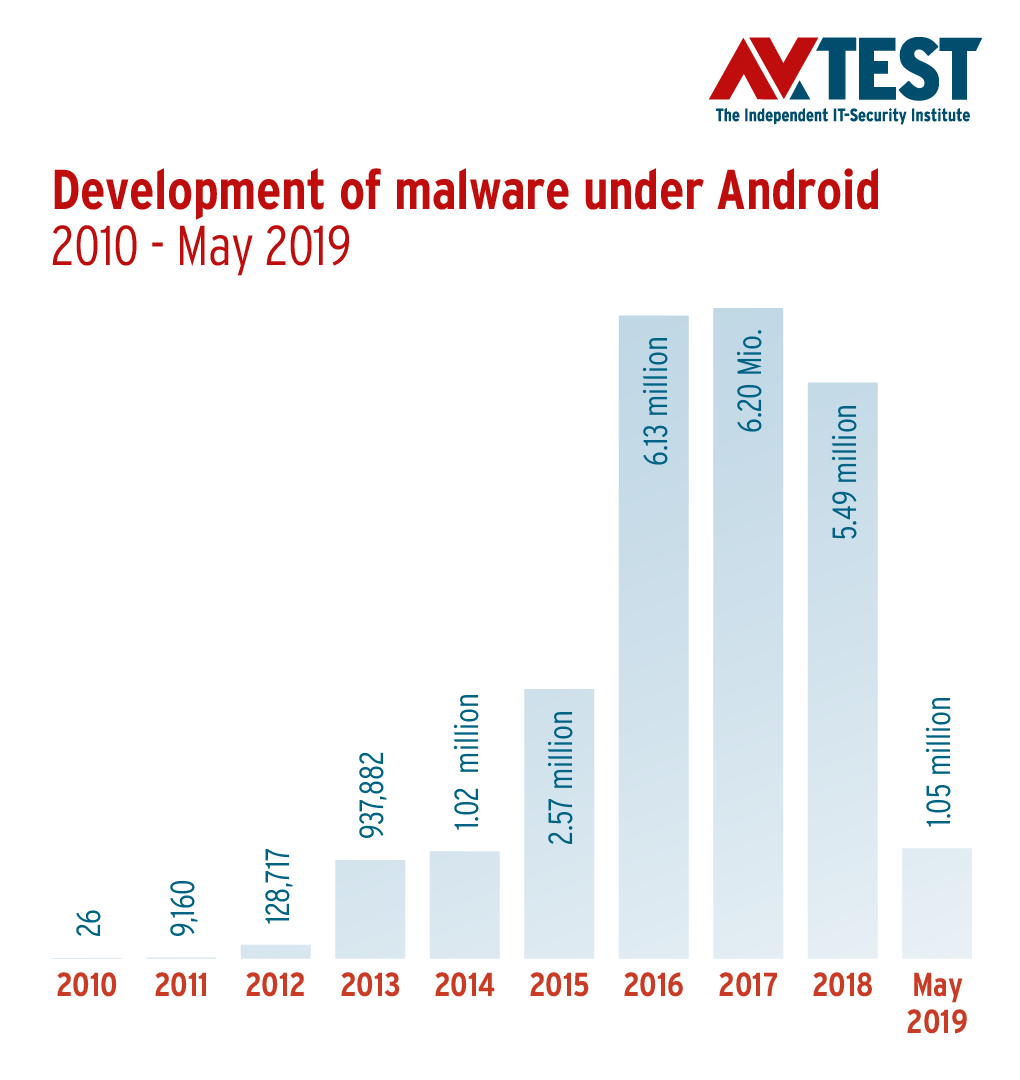
\includegraphics[scale=0.15]{img/2010-mayo2019.png}
	\caption{Nuevo malware desarrollado entre 2010 y mayo de 2019}
\end{figure}

El número de dispositivos infectados durante los dos últimos años supone una cifra preocupante:

\begin{figure}[H]
\centering
	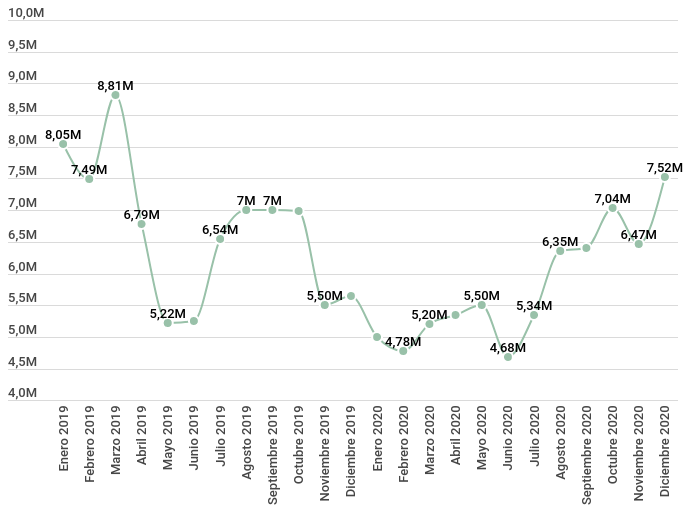
\includegraphics[scale=0.25]{img/2019-2020.png}
	\caption{2019-2020}
\end{figure}

Un indicativo de que la aplicación instalada es un malware (de cualquier tipo) es la cantidad o los tipos de permisos que requiere para su correcto funcionamiento. Las aplicaciones benignas declaran solo los permisos que de verdad necesitan, mientras que un malware declarará más permisos de los que debe y además, por lo general, serán permisos considerados peligrosos. Por ejemplo, en el caso de descargar una aplicación cuya ``funcionalidad'' es la de un bloc de notas, pero que requiere permisos para leer o envíar mensajes SMS, es altamente probable que se trate de un troyano que, o bien recoja datos y los envíe, o bien envíe mensajes que supongan un coste para el usuario.

Hay distintos tipos de análisis para detectar malware según la técnica utilizada:

\begin{itemize}
	\item \textbf{Análisis estático}: es técnica busca malware en la aplicación sin necesidad de ejecutarla. Puede utilizar técnicas de ingeniería inversa para reconstruir el código fuente y buscar comportamientos sospechosos o centrarse en los metadatos de la aplicación e intentar encontrar patrones que puedan indicar que la aplicación es maligna. Hay formas de evitar que el malware sea descubierto mediante este tipo de análisis, como por ejemplo utilizar código ofuscado (que dificulta su lectura comprimiendo y cifrando el malware, añadiendo código muerto, sustituyendo instrucciones por otras equivalentes, etc). La recolección de los permisos de una aplicación para averiguar su clasificación entra en este tipo de análisis.
	\item \textbf{Análisis dinámico}: supone la ejecución del malware en un entorno aislado y controlado (denominado \textit{sandbox environment}) que evitar que el sistema anfitrión en el que se está analizando acabe infectado. Se pueden utilizar depuradores de código para ver la ejecución paso a paso y comprobar los efectos del malware en el sistema. Al igual que en el caso del análisis estático, hay métodos para evitar que la aplicación maligna sea descubierta: detectar si se está ejecutando en un entorno virtual o si el depurador está activo, dificultar, confundir o impedir los volcados de memoria...
\end{itemize}



















